%%%%%%%%%%%%%%%%%%%%%%% file template.tex %%%%%%%%%%%%%%%%%%%%%%%%%
%
% This is a general template file for the LaTeX package SVJour3
% for Springer journals.          Springer Heidelberg 2010/09/16
%
% Copy it to a new file with a new name and use it as the basis
% for your article. Delete % signs as needed.
%
% This template includes a few options for different layouts and
% content for various journals. Please consult a previous issue of
% your journal as needed.
%
%%%%%%%%%%%%%%%%%%%%%%%%%%%%%%%%%%%%%%%%%%%%%%%%%%%%%%%%%%%%%%%%%%%
%
\RequirePackage{fix-cm}
%
%\documentclass{svjour3}                     % onecolumn (standard format)
%\documentclass[smallcondensed]{svjour3}     % onecolumn (ditto)
\documentclass[smallextended]{svjour3}       % onecolumn (second format)
%\documentclass[twocolumn]{svjour3}          % twocolumn
%
\smartqed  % flush right qed marks, e.g. at end of proof
%
\usepackage{graphicx}
%
% \usepackage{mathptmx}      % use Times fonts if available on your TeX system
%
% insert here the call for the packages your document requires
%\usepackage{latexsym}
% etc.
\usepackage{subfig}
\usepackage{graphicx}
%
% please place your own definitions here and don't use \def but
% \newcommand{}{}
%
% Insert the name of "your journal" with
% \journalname{myjournal}
%
\begin{document}

\title{Multimedia Big Data Computing with Spark on MareNostrum Supercomputer}
%\subtitle{Do you have a subtitle?\\ If so, write it here}

%\titlerunning{Short form of title}        % if too long for running head

\author{Mouna Makni \and
        Leonel Cruz \and
        Sana Imtiaz \and
        Dani Mora \and
        Mauro Gomez \and
        Jonatan Poveda \and
        Jordi Torres \and
        Ruben Tous 
}

%\authorrunning{Short form of author list} % if too long for running head

\institute{Mouna Makni, Sana Imtiaz, Dani Mora, Jordi Torres and Ruben Tous \at
              Universitat Polit\`ecnica de Catalunya (UPC). Barcelona, Spain \\
              \email{TODO}           %  \\
%             \emph{Present address:} of F. Author  %  if needed
           \and
           Leonel Cruz, Mauro Gomez and Jonatan Poveda \at
           Adsmurai. Barcelona, Spain
}

\date{Received: date / Accepted: date}
% The correct dates will be entered by the editor


\maketitle

\begin{abstract}
In this paper we describe the design and evaluation of a framework to enable multimedia Spark workloads on MareNostrum, a petascale supercomputer. As far as we know, this is the first attempt to investigate optimized deployment configurations of this kinkd of workloads on a petascale HPC setup. We present the design of the framework and evaluate the scalability of the system. We examine the impact of different configurations including parallelism, storage and networking alternatives, and we discuss several aspects in executing multimedia big data workloads on a computing system that is based on the compute-centric paradigm. We derive conclusions to facilitate systematic and optimized methodologies for fine-tuning this kind of applications on large clusters.


\keywords{Multimdia \and Big Data \and Spark \and HPC \and Instagram}
% \PACS{PACS code1 \and PACS code2 \and more}
% \subclass{MSC code1 \and MSC code2 \and more}
\end{abstract}

\section{Introduction}
\label{intro}

TODO (Ruben + help from Mouna)

\section{Related Work}
\label{sec:rw}

TODO (Ruben + help from Mouna)

\section{A framework to enable multimedia big data workloads on MareNostrum, an HPC setup}
\label{sec:spark4mn}

TODO (Ruben)

\section{Benchmarking applications}
\label{sec:exps1}

\subsection{Bag-of-Words based image classification on Instagram}

TODO (Mouna)

\begin{figure}
\centering
\subfloat{
\includegraphics[width=0.9in, height=0.9in]{img/spam1} \label{fig:ob_inflamatory_histology}}
\subfloat{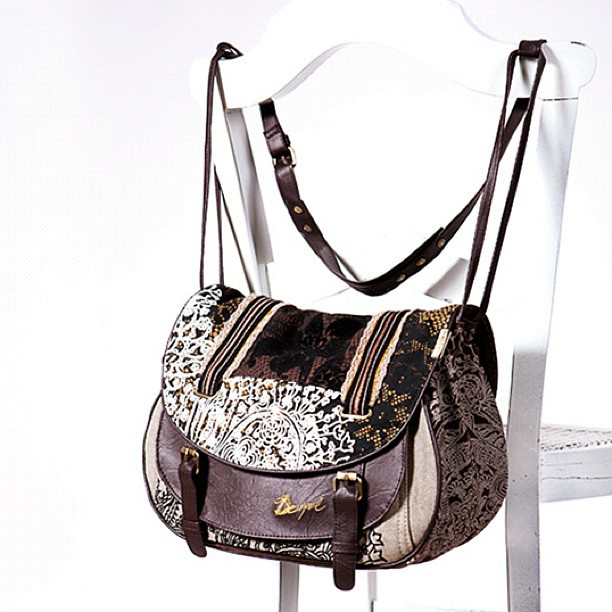
\includegraphics[width=0.9in, height=0.9in]{img/spam2} \label{fig:ob_inflamatory_histology}}
\subfloat{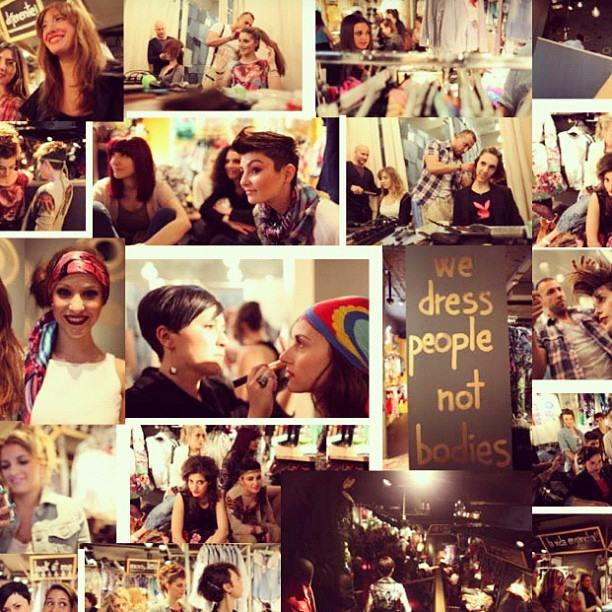
\includegraphics[width=0.9in, height=0.9in]{img/spam3} \label{fig:ob_inflamatory_histology}}\\
\subfloat{
\includegraphics[width=0.9in, height=0.9in]{img/spam4} \label{fig:ob_inflamatory_histology}}
\subfloat{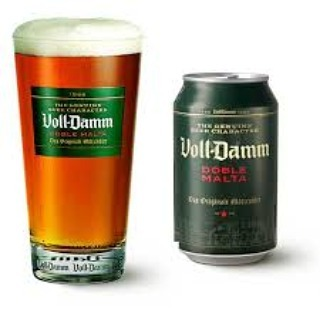
\includegraphics[width=0.9in, height=0.9in]{img/spam5} \label{fig:ob_inflamatory_histology}}
\subfloat{
\includegraphics[width=0.9in, height=0.9in]{img/spam6} \label{fig:ob_inflamatory_histology}}\\
\subfloat{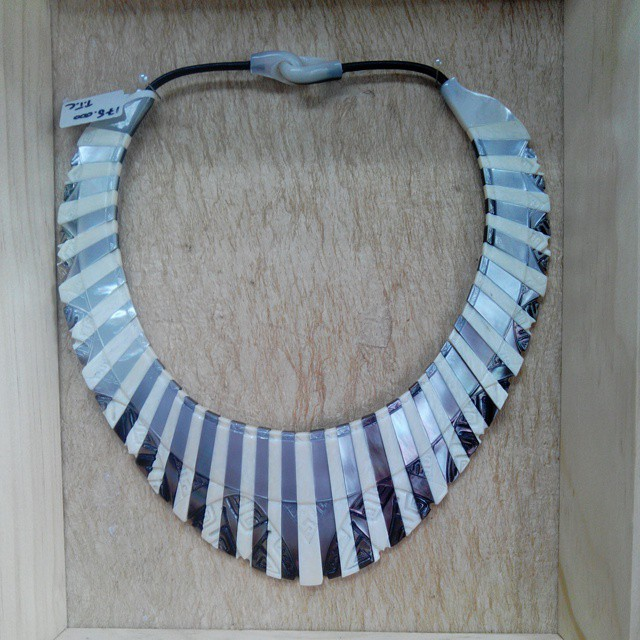
\includegraphics[width=0.9in, height=0.9in]{img/spam7} \label{fig:ob_inflamatory_histology}}
\subfloat{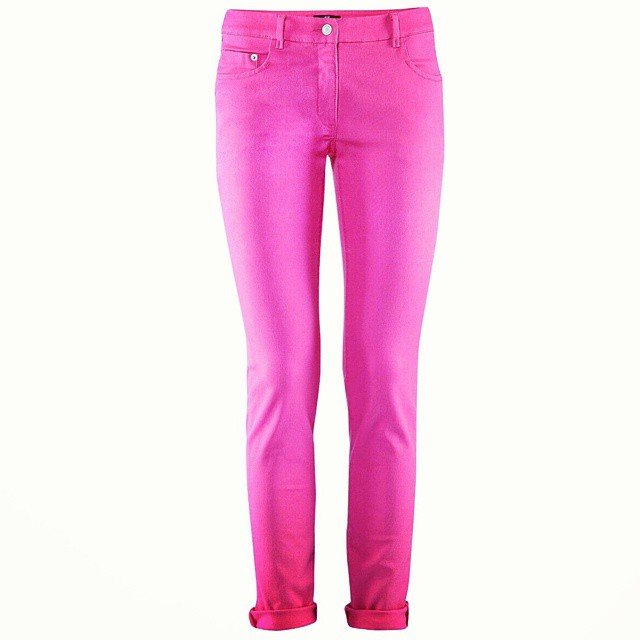
\includegraphics[width=0.9in, height=0.9in]{img/spam8} \label{fig:ob_inflamatory_histology}}
\subfloat{
\includegraphics[width=0.9in, height=0.9in]{img/spam9} \label{fig:ob_inflamatory_histology}}
\caption{Example true positives)}
\label{fig:spamexamples}
\end{figure}

\subsection{Deep convolutional networks based image classification on Instagram}

TODO (Leonel)

\subsection{Near-replica image detection on Twitter}

TODO (Dani Mora)

%
\section{Results}
%
The main goal of the experiments is to evaluate the speed-up, scale-up, and size-up properties of the proposed framework applied to the selected workloads. To this end, we use datasets up to hundreds of GBs TODO of raw data. The size of RDDs is reported to be 2-5 times larger than that; in our experiments 400GBs of data in the sort-by-key application correspond to an RDD of 1TB.
 The cluster sizes range from 8 cores up to 1024 (i.e., 64 machines)...TODO

We have submitted and tested several hundreds of jobs to MareNostrum, but we describe only the results that are of significance. Our runs include an extensive  set of configurations; for brevity, when those parameters were shown to be either irrelevant or to have negligible effect, we use default values. Each experimental configuration was repeated at least 5 times. Unless otherwise stated, we report median values in seconds. 

TODO (Ruben)

\subsection{Bag-of-Words based image classification on Instagram}

TODO (Mouna)

\subsubsection{speed-up} In the first set of experiments, we keep the input dataset constant and we increase the size of nodes/cores running the Spark application; whenever we refer to nodes, we mean  MareNostrum machines that run the executors, while the driver always runs on a separate machine; each machine is equipped with 16 cores and 32 GB of RAM. The results from 128 (8 nodes) up to 512 cores (32 nodes) are shown in Figure \ref{fig:speedup1}, where we can see that for large datasets in terms of number of records, the training can scale well. In the figure, we present the performance for the most efficient configurations; we discuss these configurations in detail later. TODO

\begin{figure}[tb!]
\begin{center}
\centerline{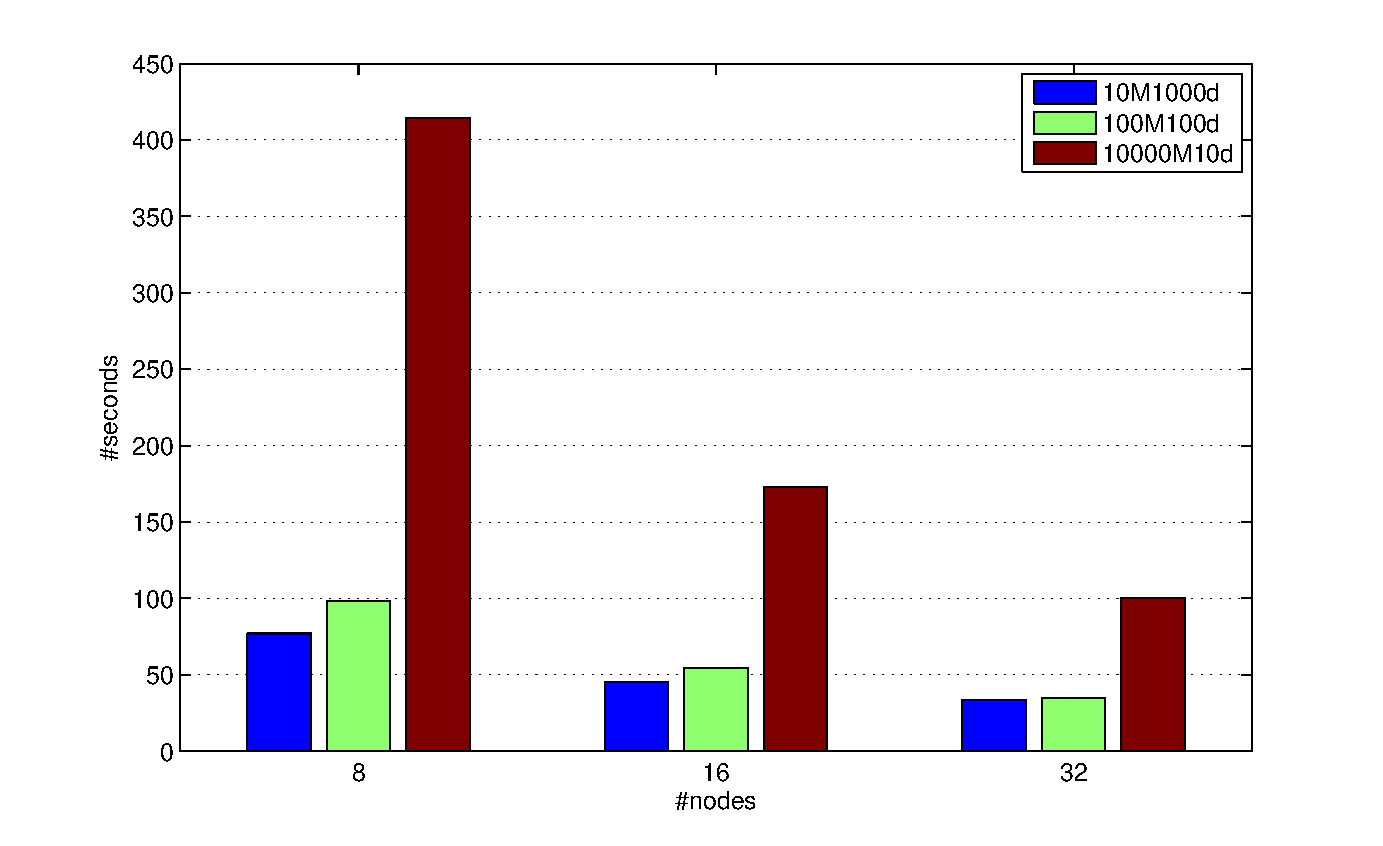
\includegraphics[width=0.75\linewidth]{img/speedup1.pdf}}
\caption{Times for training....}
\label{fig:speedup1}
\end{center}
\vspace{-0.5cm}
\end{figure}

\subsubsection{scale-up} We process the same datasets, and we now modify both the number of records and the number of machines, i.e., the infrastructure scales-out. .... The results are shown in Figure \ref{fig:scaleup1}(top). In this figure, we show both the average and the median values. Ideally, all the plots should be horizontal; our system behaves closely to that. ....

\begin{figure}[tb!]
\begin{center}
\centerline{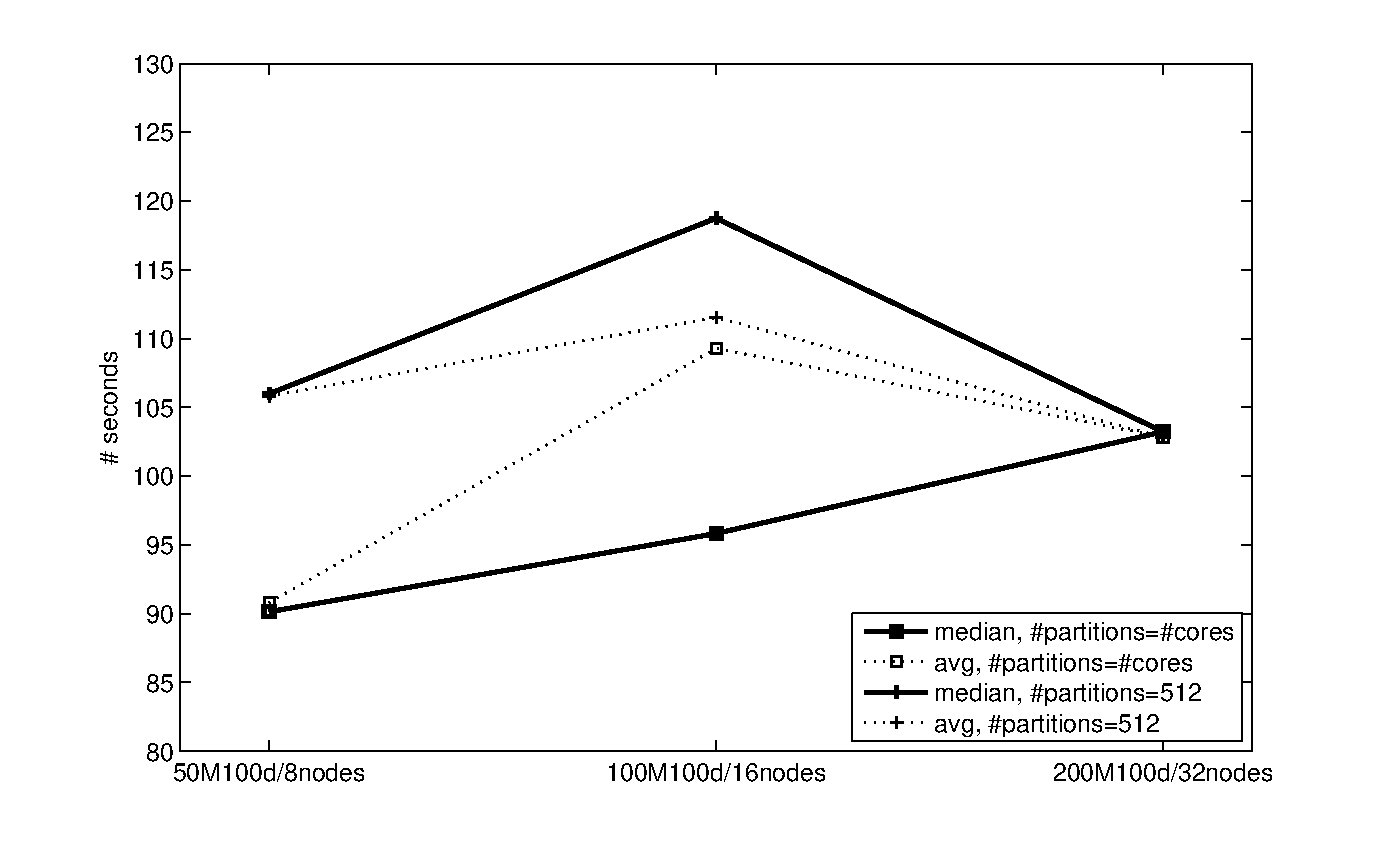
\includegraphics[width=0.75\linewidth]{img/scaleup1.pdf}}
\caption{Times for training....}
\label{fig:speedup1}
\end{center}
\vspace{-0.5cm}
\end{figure}

\subsubsection{size-up} We perform a third set of experiments, to assess the capability of sizing-up. We keep the number of nodes constant (either 16 or 32), and we gradually increase the dataset from 100GBs to 200GBs (raw data sizes). As shown in Figure \ref{fig:sizeup1}(bottom), Spark4MN exhibits a behavior where the curves are (almost) linear. ....

\begin{figure}[tb!]
\begin{center}
\centerline{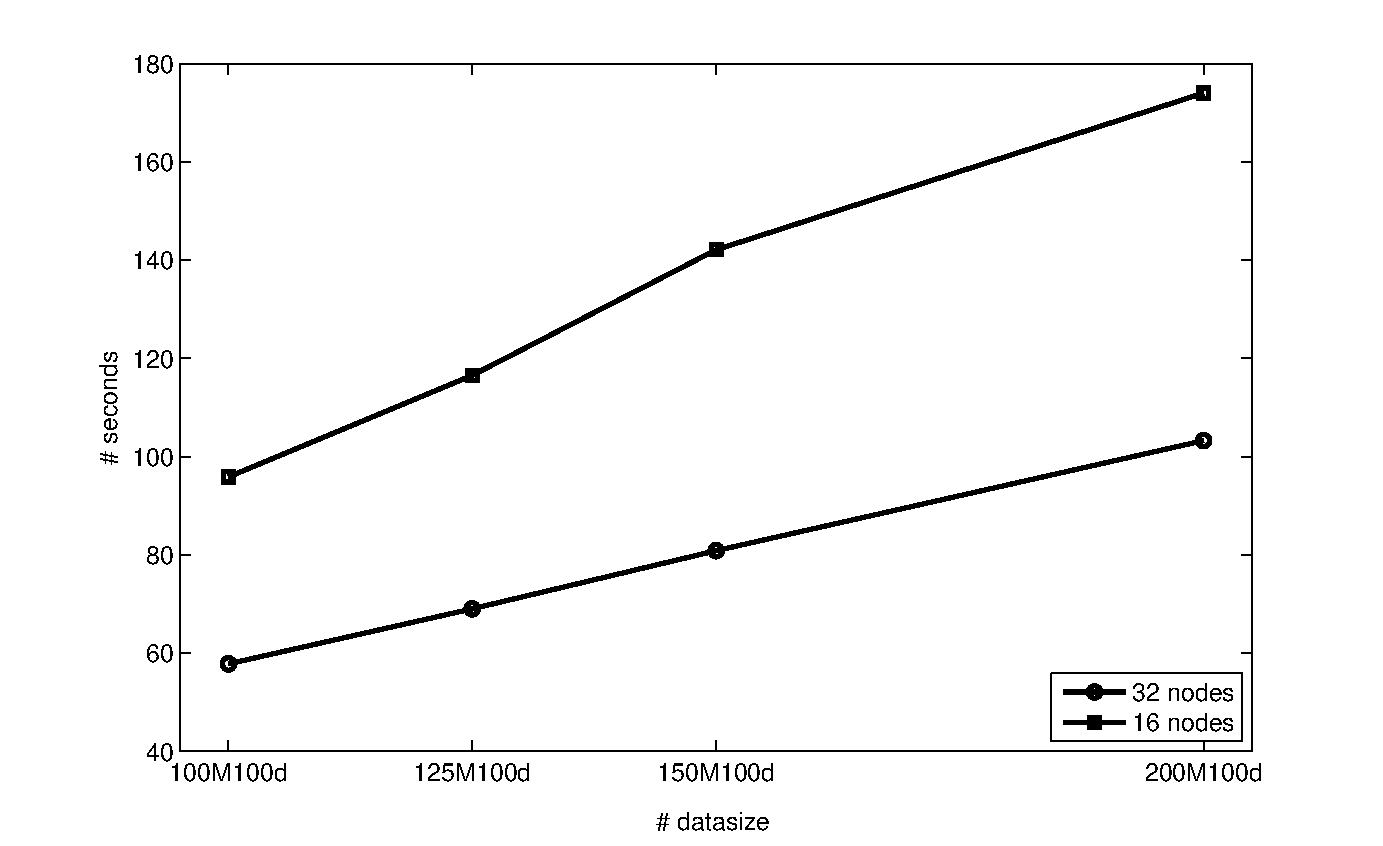
\includegraphics[width=0.75\linewidth]{img/sizeup1.pdf}}
\caption{Times for training....}
\label{fig:speedup1}
\end{center}
\vspace{-0.5cm}
\end{figure}

\subsection{Deep convolutional networks based image classification on Instagram}

TODO (Leonel)

\subsection{Near-replica image detection on Twitter}

TODO (Dani Mora)




%
\section{Conclusions}
%
The research work presented in this paper..... TODO

\begin{acknowledgements}
This work is partially supported by the Spanish Ministry of Economy and Competitivity under contract TIN2015-65316-P and by the SGR programme (2014-SGR-1051) of the Catalan Government.
\end{acknowledgements}

\bibliographystyle{spmpsci}
\bibliography{refs}

\end{document}

